
% Template:     Informe LaTeX
% Documento:    Archivo principal
% Versión:      8.1.6 (12/06/2022)
% Codificación: UTF-8
%
% Autor: Pablo Pizarro R.
%        pablo@ppizarror.com
%
% Manual template: [https://latex.ppizarror.com/informe]
% Licencia MIT:    [https://opensource.org/licenses/MIT]

% CREACIÓN DEL DOCUMENTO
\documentclass[
	spanish, % Idioma: spanish, english, etc.
	letterpaper, oneside
]{article}

\usepackage{svg}
%\usepackage[inkscapelatex=false]{svg}

% INFORMACIÓN DEL DOCUMENTO
\def\documenttitle {[PENDING-TITLE].}
\def\documentsubtitle {}
\def\documentsubject {[NO-CODE] [PENDING-SUBTITLE]}

\def\documentauthor {Diego Peña Loza, Roberto Guajardo M.}
\def\coursename {Introducción al Procesamiento Digital de Imágenes}
\def\coursecode {[NO-CODE]}

\def\universityname {Universidad de Chile}
\def\universityfaculty {Facultad de Ciencias Físicas y Matemáticas}
\def\universitydepartment {Departamento de Ingeniería Eléctrica}
\def\universitydepartmentimage {departamentos/die}
\def\universitydepartmentimagecfg {height=1.57cm}
\def\universitylocation {Santiago de Chile}

% INTEGRANTES, PROFESORES Y FECHAS
\def\authortable {
\begin{tabular}{ll}
	Integrantes:
	& \begin{tabular}[t]{l}
		Diego Peña Loza \\
        Roberto Guajardo M.
	\end{tabular} \\
	Profesor:
	& \begin{tabular}[t]{l}
		Constanza Ahumada
	\end{tabular} \\
    Encargados de Laboratorio:
	& \begin{tabular}[t]{l}
		[PENDING].
	\end{tabular} \\

	& \\
    \\
	\multicolumn{2}{l}{\universitylocation}
\end{tabular}
}

% IMPORTACIÓN DEL TEMPLATE
\input{template}

% INICIO DE PÁGINAS
\begin{document}
	
% PORTADA
\templatePortrait

% CONFIGURACIÓN DE PÁGINA Y ENCABEZADOS
\templatePagecfg

% RESUMEN O ABSTRACT
%\begin{abstractd}
	%\lipsum[1] % Párrafo ejemplo, se puede borrar
%\end{abstractd}

% TABLA DE CONTENIDOS - ÍNDICE
\templateIndex

% CONFIGURACIONES FINALES
\templateFinalcfg

% ======================= INICIO DEL DOCUMENTO =======================

%\section{Objetivos y tareas a realizar} \label{sec:tareas}
%\input{sections/tareas}

\newpage
\section{Introducción}

El propósito del presente informe es entregar una guía de apoyo para comprender como se realizó la modificación del montaje del motor de corriente continua. Anteriormente este contaba solamente con un motor de corriente continua y la única variable medida era la velocidad rotacional del eje del motor. Dada la necesidad de implementar un sistema de lazos anidados y además de aplicar una carga mecánica que ejerza torque al motor eléctrico, se implementó un sistema de medición de corriente para poder comunicar la corriente de armadura que consume el motor DC con el programa que realiza el control, se acopló mecánicamente un generador eléctrico, y, además, se implementó un módulo de carga electrónica conectada a la armadura del generador que permite ser controlado desde el computador para aumentar o disminuir la carga del generador.\\

En las siguientes secciones se deescribirá en detalle como se conforma el sistema completo, tanto a nivel físico como computacional, y también, como se implementaron todas las adiciones.\\

\section{Setup físico}

A continuación, se presenta una descripción general de la conexión entre los módulos del setup, utilizando diagramas de bloques como apoyo.

\subsection{Descripción del setup físico}

El setup físico consta de un motor eléctrico acoplado mecánicamente a un generador eléctrico. Ambos son máquinas de corriente continua con dos terminales para la excitación de campo y dos terminales para el acceso a la armadura. Para controlar el motor eléctrico, se utiliza un computador con sistema operativo Windows y el software Simulink, perteneciente a la familia de MATLAB. Este software permite implementar las estrategias de control aplicadas a las máquinas.

La comunicación entre el computador y el sistema físico se realiza mediante un módulo comercial OPTO-22. Este módulo establece una comunicación por protocolo Ethernet, formando una red directa entre el computador y el OPTO-22 mediante un cable Ethernet. La Figura \ref{fig:esquema} muestra un diagrama global del setup.

\begin{figure}[H]
    \centering
    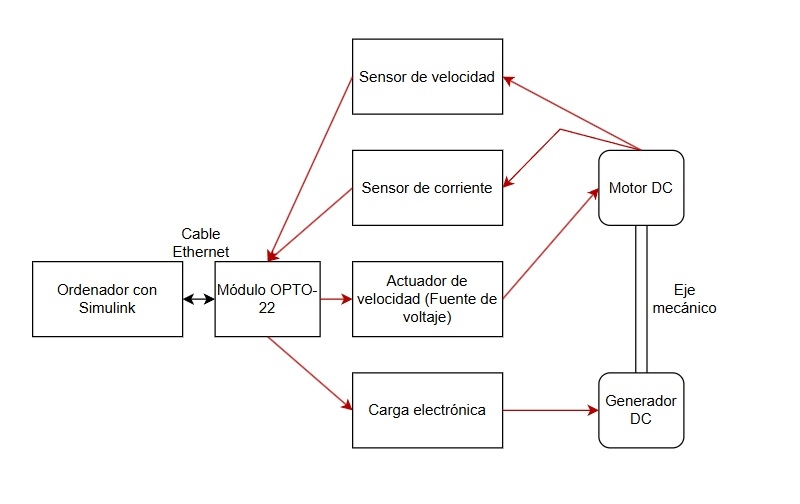
\includegraphics[width=0.75\linewidth]{img/diagramaGlobal.jpg}
    \caption{Esquema completo del sistema}
    \label{fig:esquema}
\end{figure}

\subsection{Componentes del setup}

El sistema implementado está compuesto por distintos módulos electrónicos y computacionales que permiten realizar el control, la adquisición de datos y la aplicación de carga sobre la máquina de corriente continua. Cada componente cumple una función específica dentro del lazo de control y adquisición del sistema. A continuación, se describe el propósito y funcionamiento general de cada uno de ellos.

\subsubsection{Módulo OPTO-22}

El módulo OPTO-22 corresponde a la interfaz principal entre el computador y el sistema físico. 
Este dispositivo permite adquirir señales analógicas provenientes de sensores y, además, 
generar señales analógicas de control hacia los actuadores del sistema. Para realizar su funcion, requiere de una alimentacion de 5 Vdc.\\

La comunicación entre el computador y el módulo OPTO-22 (ver Figura \ref{fig:OPTO22}) se realiza mediante protocolo Ethernet, 
estableciendo una red directa entre ambos dispositivos. Desde Simulink se envían comandos de voltaje hacia el motor y la carga electrónica, 
mientras que el OPTO-22 retorna las mediciones de velocidad y corriente para ser utilizadas posteriormentepor los algoritmos de control.

\begin{figure}[H]
    \centering
    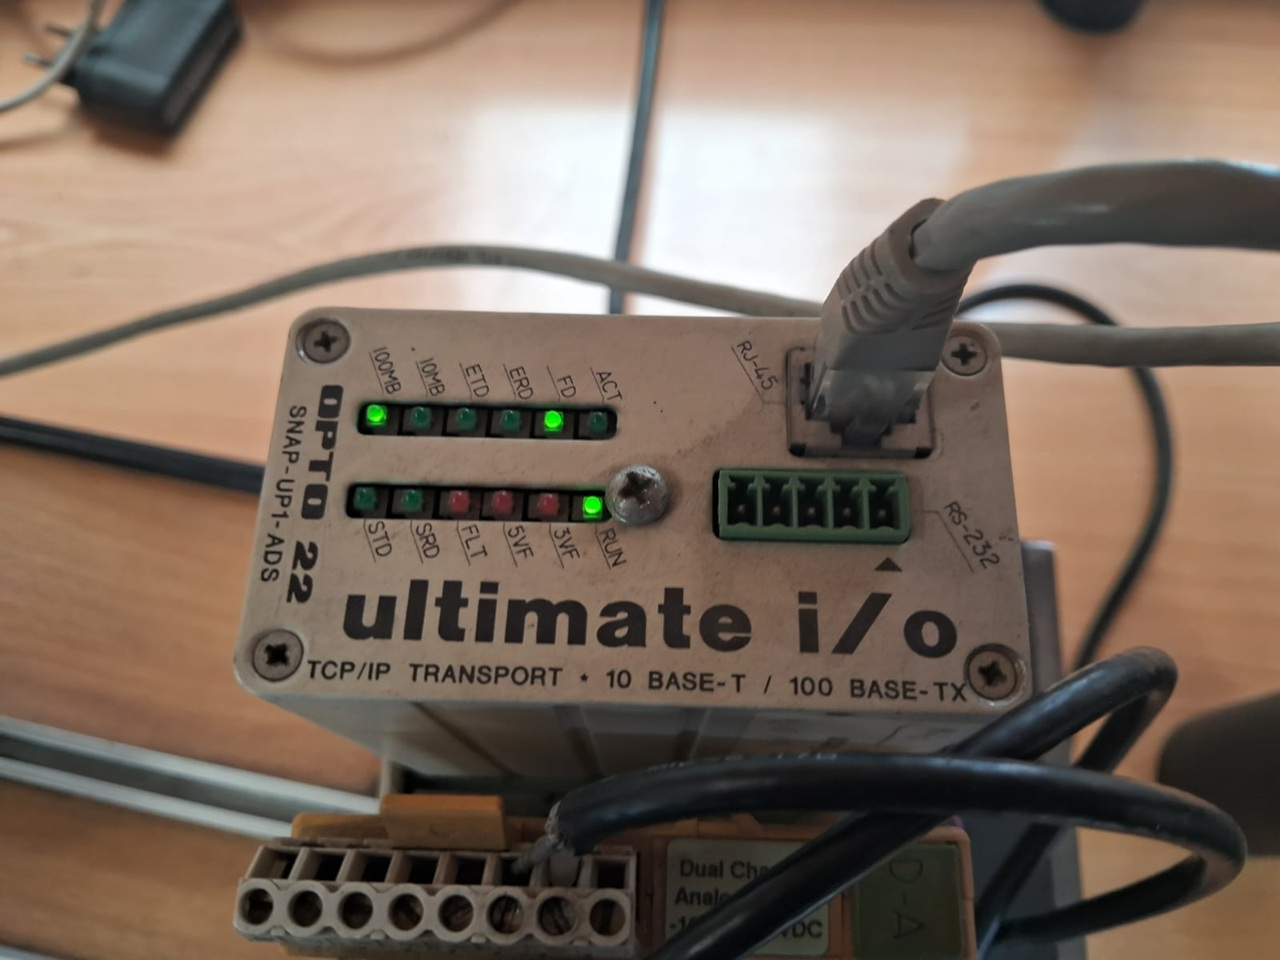
\includegraphics[width=0.75\linewidth]{img/OPTO22.jpg}
    \caption{Vista del OPTO22}
    \label{fig:OPTO22}
\end{figure}


En la implementación actual se utilizan los módulos SNAP-AOV-27 para las salidas analógicas y SNAP-AIV-4 para las entradas analógicas (ver Figura \ref{fig:snap}. Los rangos de voltaje que soportan ambos modulos son de -10 a 10 V de forma continua.


\begin{figure}[H]
    \centering
    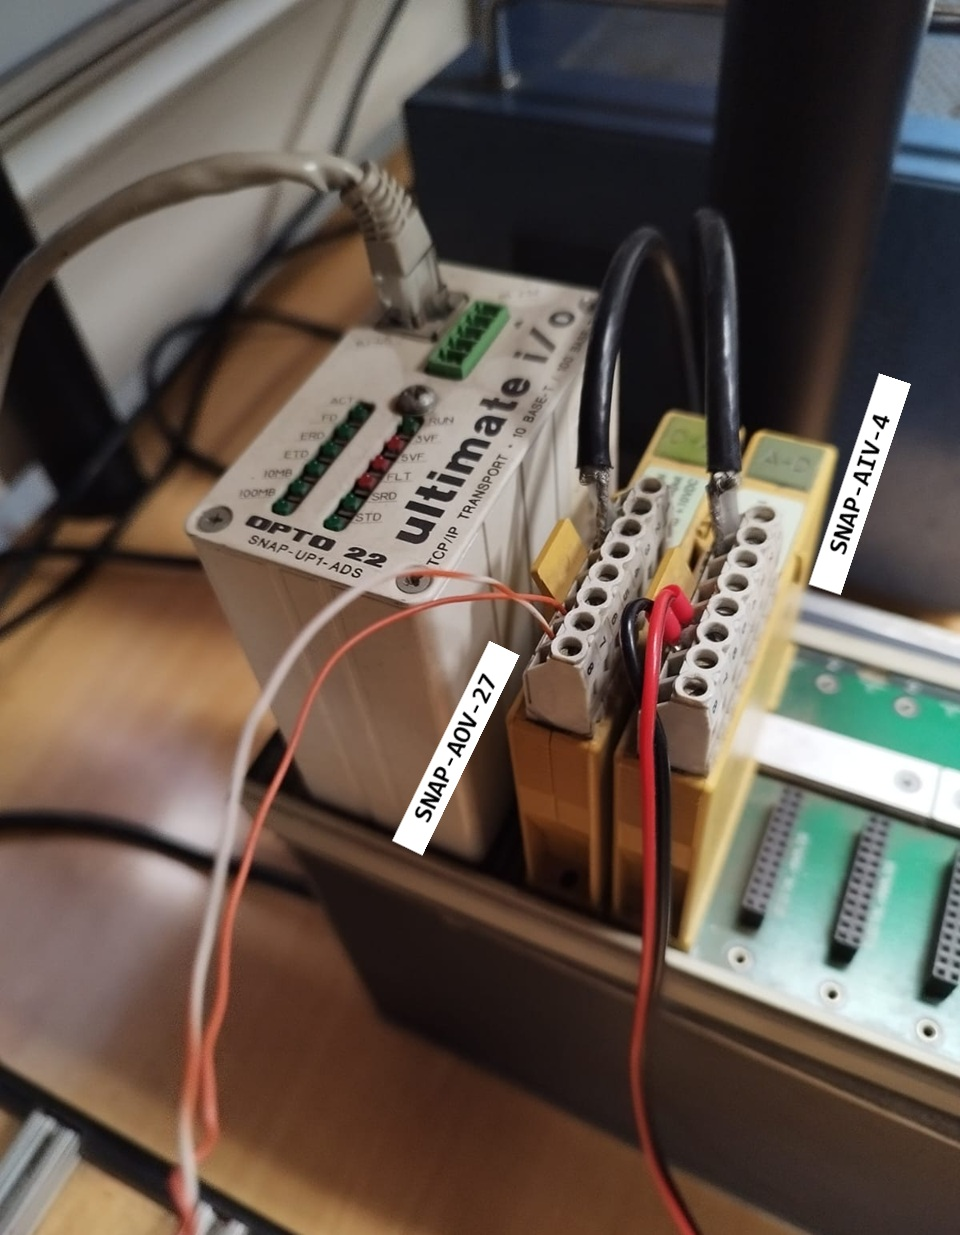
\includegraphics[width=0.75\linewidth]{img/snap.jpg}
    \caption{Vista de los modulos de entradas y salidas analogicas SNAP-AIV-4 y SNAP-AOV-27 respectivamente}
    \label{fig:snap}
\end{figure}

NOTA: La alimentacion de 5 Vdc necesaria para alimentar el modulo OPTO-22 proviene del Actuador de velocidad.

\subsubsection{Actuador de velocidad}

El actuador de velocidad es el modulo mostrado en la siguiente Figura \ref{fig:ActV}. 

\begin{figure}[H]
    \centering

    \subfloat[Primera imagen.\label{fig:ActV1}]{
        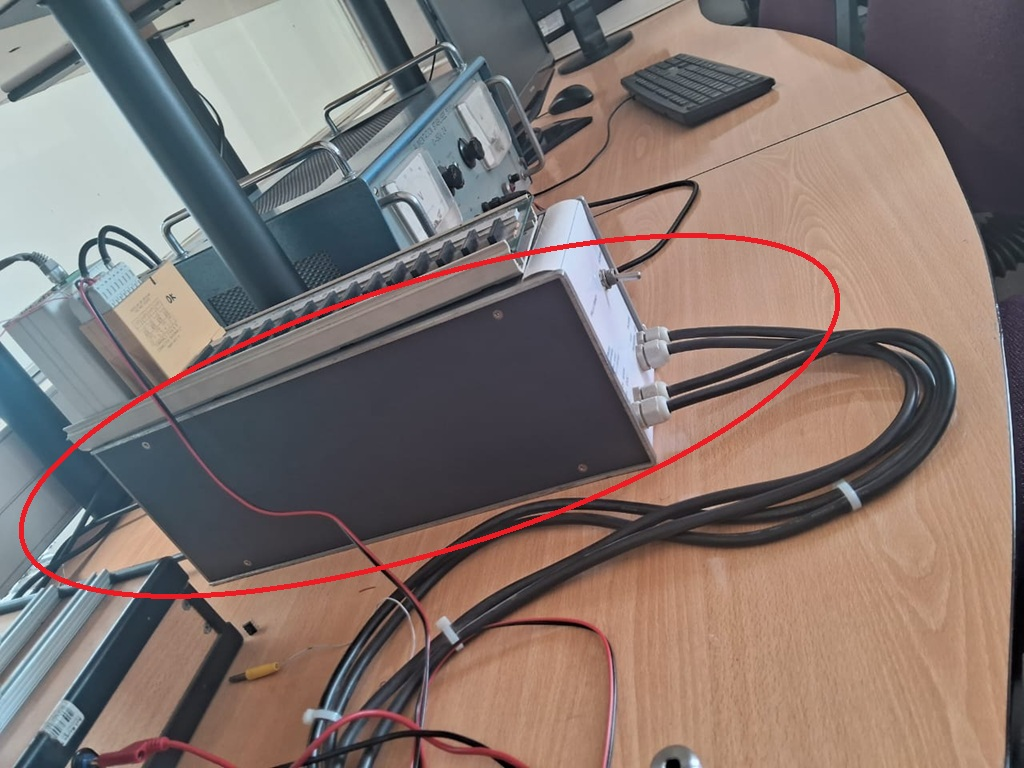
\includegraphics[width=0.5\textwidth]{img/ActV1.jpg}
    }
    \hfill
    \subfloat[Segunda imagen.\label{fig:ActV2}]{
        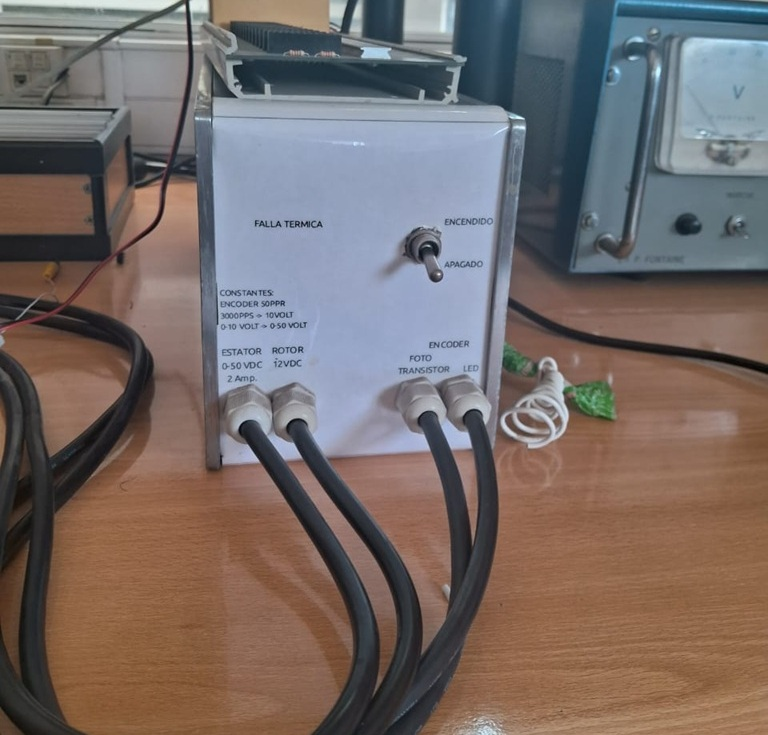
\includegraphics[width=0.5\textwidth]{img/ActV2.jpg}
    }

    \caption{Comparación entre ambas imágenes.}
    \label{fig:ActV}
\end{figure}

Dicho modulo recibe la señal de velocidad enviada desde Simulink mediante OPTO-22 a través del módulo de salidas analógicas SNAP-AOV-27, y, le aplica una amplificación de voltaje de un factor de aproximadamente 4, además, le agrega una etapa de potencia a la señal para ser aplicada a los bornes de la armadura del motor (lo cuál demanda un consumo de corriente). El funcionamiento interno del actuador se desconoce, pero se presume que puede ser un amplificador de voltaje seguido un amplificador de corriente para otorgar potencia al motor.

NOTA: Este modulo se alimenta mediante una fuente de 50 Vdc.

\subsubsection{Sensor de velocidad}

La velocidad angular del motor se mide mediante un sensor de velocidad basado en un disco con agujeros acoplado al eje del motor y un foto transistor acoplado opticamente con un diodo led infrarrojo los cuales al quedar alineados con un agujero del disco activan un 1 logico, lo que genera una señal con cierta frecuencia que permite determinar la velocidad rotacional del motor. Ver Figura \ref{fig:Encoder}.

\begin{figure}[H]
    \centering
    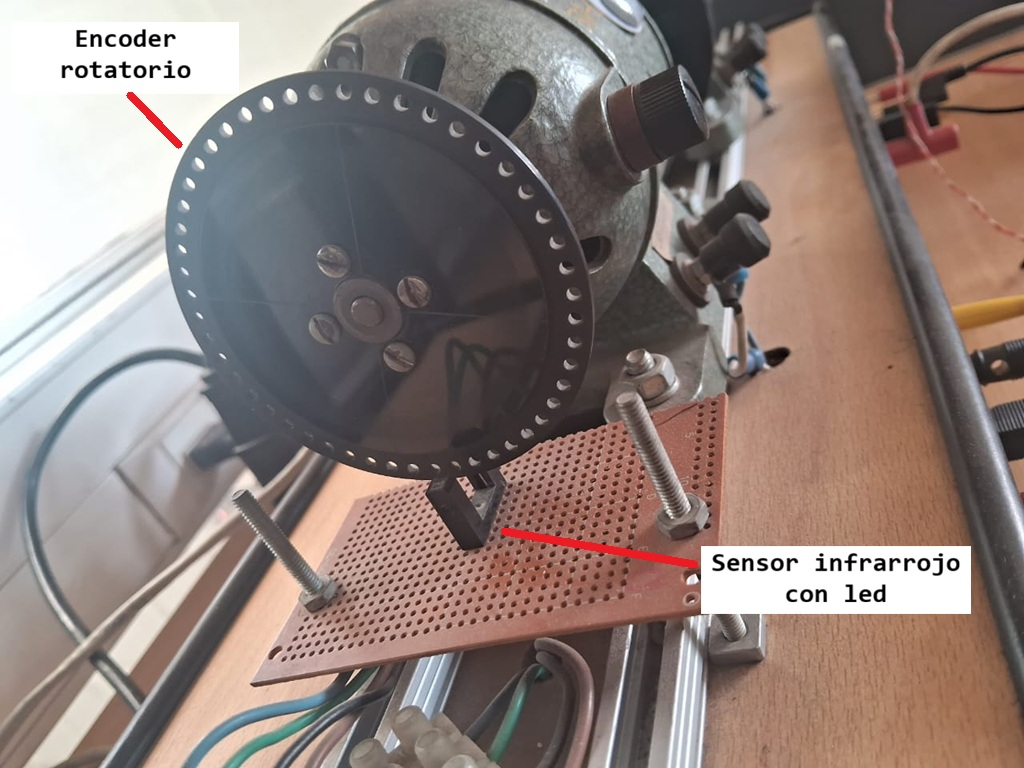
\includegraphics[width=0.75\linewidth]{img/Encoder.jpg}
    \caption{Vista del Encoder}
    \label{fig:Encoder}
\end{figure}

Dicha señal pulsante se envía al módulo que contiene al actuador de velocidad (ver Figura \ref{fig:ActV}), para ser transformada a un voltaje proporcional a la velocidad rotacional del eje mecánico del motor. Esta señal continua es enviada al módulo OPTO-22 mediante el módulo de entradas analógicas SNAP-AIV-4 para ser digitalizada y procesada en Simulink.

NOTA: La cantidad de agujeros que posee el disco se desconoce, pues no es necesario ya que dicha labor se encuentra correctamente implementada. 

\subsubsection{Sensor de corriente}

Con el fin de medir la corriente de armadura consumida por el motor, se implementó una PCB dedicada (más detalles en la seccion 'Solucion') basada en el sensor LA 55-P. 
Este sensor permite realizar mediciones de corriente con aislamiento eléctrico y sin intervenir directamente el circuito de potencia.

La señal entregada por el sensor es acondicionada mediante amplificadores operacionales y circuitos limitadores para obtener un rango compatible con las entradas analógicas del OPTO-22. Por último, al igual que el sensor de velocidad, la señal de corriente es entregada como voltaje analógico al módulo SNAP-AIV-4. \\

Nota: El módulo de medición de corriente también puede utilizarse para otros tipos de mediciones, por ejemplo, la corriente de campo del motor.

\subsubsection{Carga electrónica}
La carga electrónica fue diseñada con el propósito de aplicar una carga variable sobre el generador DC acoplado mecánicamente al motor  (más detalles en la seccion 'Solucion'). 
Esto permite simular distintas condiciones de carga y evaluar el comportamiento dinámico del sistema bajo diferentes exigencias. \\

La carga es controlada mediante una señal analógica proveniente del OPTO-22 (salida desde el módulo SNAP-AOV-27), permitiendo variar la corriente consumida por el circuito de potencia.
Internamente, la etapa de disipación utiliza un transistor TIP41C montado sobre un disipador térmico.



\newpage 
\section{Código SDCMotor}
\label{sec:codigo_SDCMotor}
\subsection{Propósito y alcance}
El archivo \texttt{SDCMotor.cpp} implementa una \emph{S-Function Level-2} para Simulink cuyo objetivo es actuar como puente entre el modelo de control y un módulo de E/S analógicas OPTO22 (vía Ethernet), utilizando la librería \texttt{O22SIOMM} (clase \texttt{O22SnapIoMemMap}). En cada paso de simulación el bloque:
\begin{itemize}
    \item \textbf{envía} al OPTO22 dos comandos analógicos: comando de voltaje para el actuador, y  una corriente de carga (\texttt{iLoad})\footnote{El significado físico exacto depende de la conexión real.};
    \item \textbf{recibe} desde el OPTO22 dos mediciones analógicas:  velocidad (\texttt{velocidad}) y  corriente (\texttt{corriente});
    \item \textbf{detiene} la simulación si se acumulan demasiados errores de comunicación.
\end{itemize}



\subsubsection{Red y configuración fija en el código}
La S-Function abre la comunicación Ethernet con un \emph{Brain} OPTO22 en la IP \texttt{192.168.6.101} y puerto \texttt{2001}. Por lo tanto, el PC y el equipo OPTO22 deben estar en la misma red/subred y sin bloqueo por firewall/ACL. (Estos valores están embebidos en \texttt{SDCMotor.cpp}; si se cambia el setup, deben actualizarse en el código o parametrizarse.)

\subsubsection{Requisitos de compilación (MEX/S-Function)}
Para generar el binario \texttt{SDCMotor.mex*} se requiere:
\begin{itemize}
    \item \textbf{Un compilador C/C++ soportado por MATLAB} configurado con \texttt{mex -setup C++}.
    \item \textbf{Headers y librería} de OPTO22 (\texttt{O22SIOMM.h} y la correspondiente \texttt{.lib/.dll} o fuentes) disponibles en rutas conocidas.
\end{itemize}
MATLAB permite especificar rutas de \emph{include} con \texttt{-I} y enlazado con opciones de librería durante \texttt{mex}.

\subsubsection{Compilación recomendada desde MATLAB}
Desde la carpeta donde reside \texttt{SDCMotor.cpp}, compilar preferentemente con:
\begin{verbatim}
mex -v SDCMotor.cpp ...
    -I"<RUTA_OPTO22>\include" ...
    -L"<RUTA_OPTO22>\lib" -lO22SIOMM
\end{verbatim}

\noindent Si la distribución de OPTO22 entrega la implementación como fuentes (por ejemplo, \texttt{O22SIOMM.cpp}), una alternativa directa es:
\begin{verbatim}
mex -v SDCMotor.cpp O22SIOMM.cpp -I"<RUTA_OPTO22>\include"
\end{verbatim}

\noindent Tras compilar, el archivo \texttt{SDCMotor.mex*} debe quedar en el \emph{MATLAB path} o en el mismo directorio del modelo para que Simulink pueda cargar el bloque.

\subsection{Dependencias y compilación}
\begin{itemize}
    \item \textbf{API Simulink:} \texttt{simstruc.h} para la definición de S-Functions.
    \item \textbf{OPTO22:} \texttt{O22SIOMM.h} y la implementación asociada de la librería (debe estar disponible al compilar el MEX).
\end{itemize}

\noindent La S-Function se declara como:
\begin{verbatim}
#define S_FUNCTION_NAME  SDCMotor
#define S_FUNCTION_LEVEL 2
\end{verbatim}
y se encapsula en \texttt{extern C} para asegurar \emph{linkage} compatible con el mecanismo de carga de Simulink.

\subsection{Parámetros del bloque}
El bloque define \textbf{un (1) parámetro} de máscara:
\begin{itemize}
    \item \textbf{P1:} tiempo de muestreo $T_s$ (segundos). Se lee en \texttt{mdlInitializeSampleTimes()} mediante:
    \[
        T_s \leftarrow \texttt{mxGetScalar(ssGetSFcnParam(S,0))}
    \]
\end{itemize}
Si la cantidad de parámetros provistos en Simulink no coincide con lo esperado, \texttt{mdlInitializeSizes()} retorna y Simulink reporta el error.

\subsection{Interfaz de entradas y salidas}
El bloque tiene \textbf{2 entradas escalares} y \textbf{2 salidas escalares}, todas tipo \texttt{real\_T}:

\begin{table}[h]
\centering
\begin{tabular}{lll}
\hline
\textbf{Puerto} & \textbf{Señal} & \textbf{Descripción} \\
\hline
Entrada 0 & $u$      & Comando de voltaje a enviar al OPTO22 (canal analógico 0). \\
Entrada 1 & $iLoad$  & Corriente de carga a enviar al OPTO22 (canal analógico 1). \\
\hline
Salida 0 & $y$      & Velocidad leída desde OPTO22 (canal analógico 4). \\
Salida 1 & $z$      & Corriente leída desde OPTO22 (canal analógico 6). \\
\hline
\end{tabular}
\caption{Mapa de puertos de Simulink a puntos analógicos OPTO22.}
\label{tab:sdcmotor_ports}
\end{table}

\noindent Además, se exige memoria contigua para ambas entradas (\texttt{ssSetInputPortRequiredContiguous}), lo que simplifica el acceso a las señales.

\subsection{Vectores de trabajo y estados}
Para mantener información entre llamados, la S-Function reserva:
\begin{itemize}
    \item \textbf{PWork (1 puntero):} almacena un puntero a la instancia \texttt{O22SnapIoMemMap} que representa la conexión activa con el OPTO22.
    \item \textbf{IWork (1 entero):} contador de errores de comunicación (\texttt{WORK\_INT\_ERROR\_COUNT}).
\end{itemize}
Se define además \textbf{1 estado discreto} (\texttt{ssSetNumDiscStates(S,1)}), aunque en esta implementación no se observa uso explícito de \texttt{ssGetX}/\texttt{ssSetX}; en la práctica, la memoria persistente relevante queda cubierta por \texttt{PWork} e \texttt{IWork}.

\subsection{Manejo de errores}
El bloque implementa un mecanismo simple de tolerancia a fallos:
\begin{itemize}
    \item Cada vez que una operación de lectura/escritura hacia OPTO22 retorna un código distinto de \texttt{SIOMM\_OK}, se incrementa \texttt{IWork[ERROR\_COUNT]} y se imprime un mensaje vía \texttt{ssPrintf}.
    \item Si el contador supera \texttt{MAX\_ERROR\_COUNT} (definido como 5), se invoca \texttt{ssSetErrorStatus(S, "...")} y Simulink detiene la ejecución del modelo.
\end{itemize}

\subsection{Ciclo de vida del bloque (funciones S-Function)}
A continuación se describe el rol de cada función obligatoria/registrada y el flujo típico en simulación.

\subsubsection{\texttt{mdlInitializeSizes(S)}: declaración de capacidades}
Configura la firma del bloque: número de parámetros, puertos de entrada/salida, tiempos de muestreo y tamaños de vectores de trabajo. En particular:
\begin{itemize}
    \item 1 parámetro esperado.
    \item 2 entradas escalares y 2 salidas escalares.
    \item 1 tiempo de muestreo.
    \item \texttt{PWork} para el objeto de interfaz OPTO22 y \texttt{IWork} para el contador de errores.
\end{itemize}

\subsubsection{\texttt{mdlInitializeSampleTimes(S)}: tiempo de muestreo}
Asigna el tiempo de muestreo del bloque a partir del parámetro $T_s$ y fija offset en 0:
\[
    T_s = \texttt{Param(0)}, \qquad \text{offset} = 0.
\]

\subsubsection{\texttt{mdlStart(S)}: apertura de conexión con OPTO22}
Se ejecuta una sola vez al inicio. Sus pasos son:
\begin{enumerate}
    \item Crea el objeto \texttt{Brain = new O22SnapIoMemMap()}.
    \item Abre conexión Ethernet con:
    \begin{itemize}
        \item IP: \texttt{192.168.6.101}
        \item Puerto: \texttt{2001}
        \item Timeout: \texttt{10000} (ms)
        \item Último argumento: \texttt{1} (dependiente de la API; típicamente flags/modo).
    \end{itemize}
    \item Espera a que la apertura finalice consultando \texttt{IsOpenDone()} mientras retorne 
    
    \texttt{SIOMM\_ERROR\_NOT\_CONNECTED\_YET}.
    \item Si ocurre un error, define un estado de error fatal:
    \begin{center}
        \texttt{"Unable to connect to OPTO22 (192.168.6.101)."}
    \end{center}
    \item Si la conexión es exitosa, guarda el puntero del objeto en \texttt{ssGetPWork(S)[0]} e inicializa el contador de errores en 0.
\end{enumerate}

\subsubsection{\texttt{mdlUpdate(S,tid)}: escritura de comandos (salida hacia planta)}
En cada paso de simulación, el bloque toma las entradas de Simulink y las envía al OPTO22:
\begin{itemize}
    \item Entrada 0 ($u$) $\rightarrow$ \texttt{SetAnaPtValue(0, (float)*u)}.
    \item Entrada 1 ($iLoad$) $\rightarrow$ \texttt{SetAnaPtValue(1, (float)*iLoad)}.
\end{itemize}
Cada envío es verificado; ante error se incrementa el contador y, si se supera el umbral, se detiene la simulación.

\paragraph{Nota.}
El mensaje impreso ante error en el segundo envío repite el texto \texttt{Error sending voltage command.\textbackslash n}; si se quiere mayor trazabilidad, se puede diferenciar mensajes (p.ej. ``voltage'' vs ``load current'').

\subsubsection{\texttt{mdlOutputs(S,tid)}: lectura de mediciones (entrada desde planta)}
En cada paso, el bloque consulta dos valores analógicos:
\begin{itemize}
    \item Velocidad: \texttt{GetAnaPtValue(4, \&velocidad)} $\rightarrow y = \texttt{(real\_T)velocidad}$.
    \item Corriente: \texttt{GetAnaPtValue(6, \&corriente)} $\rightarrow z = \texttt{(real\_T)corriente}$.
\end{itemize}
Las lecturas tienen la misma política de manejo de errores descrita previamente.

\subsubsection{\texttt{mdlTerminate(S)}: cierre seguro}
Al terminar la simulación:
\begin{enumerate}
    \item Recupera el objeto desde \texttt{PWork}.
    \item Envía \textbf{0.0} al canal analógico 0 (\texttt{SetAnaPtValue(0,0.0)}) como acción de seguridad para dejar el comando de voltaje en cero.
    \item \hl{\textbf{AGREGAR: Brain->SetAnaPtValue(1,0.0); para cierre seguro del nuevo canal!!!!!!!}}
    \item Cierra la conexión (\texttt{Close()}).
    \item Libera memoria (\texttt{delete Brain}).
\end{enumerate}

\subsection{Resumen operacional (pseudoflujo)}
\begin{verbatim}
Start:
  conectar a OPTO22 (IP fija)
  error_count = 0

Cada Ts:
  mdlUpdate:
    enviar u -> AO0
    enviar iLoad -> AO1
  mdlOutputs:
    leer velocidad <- AI4
    leer corriente <- AI6
  si error_count > 5:
    detener simulación

Terminate:
  AO0 = 0
  AO1 = 0
  cerrar conexión
\end{verbatim}

\begin{figure}
    \centering
    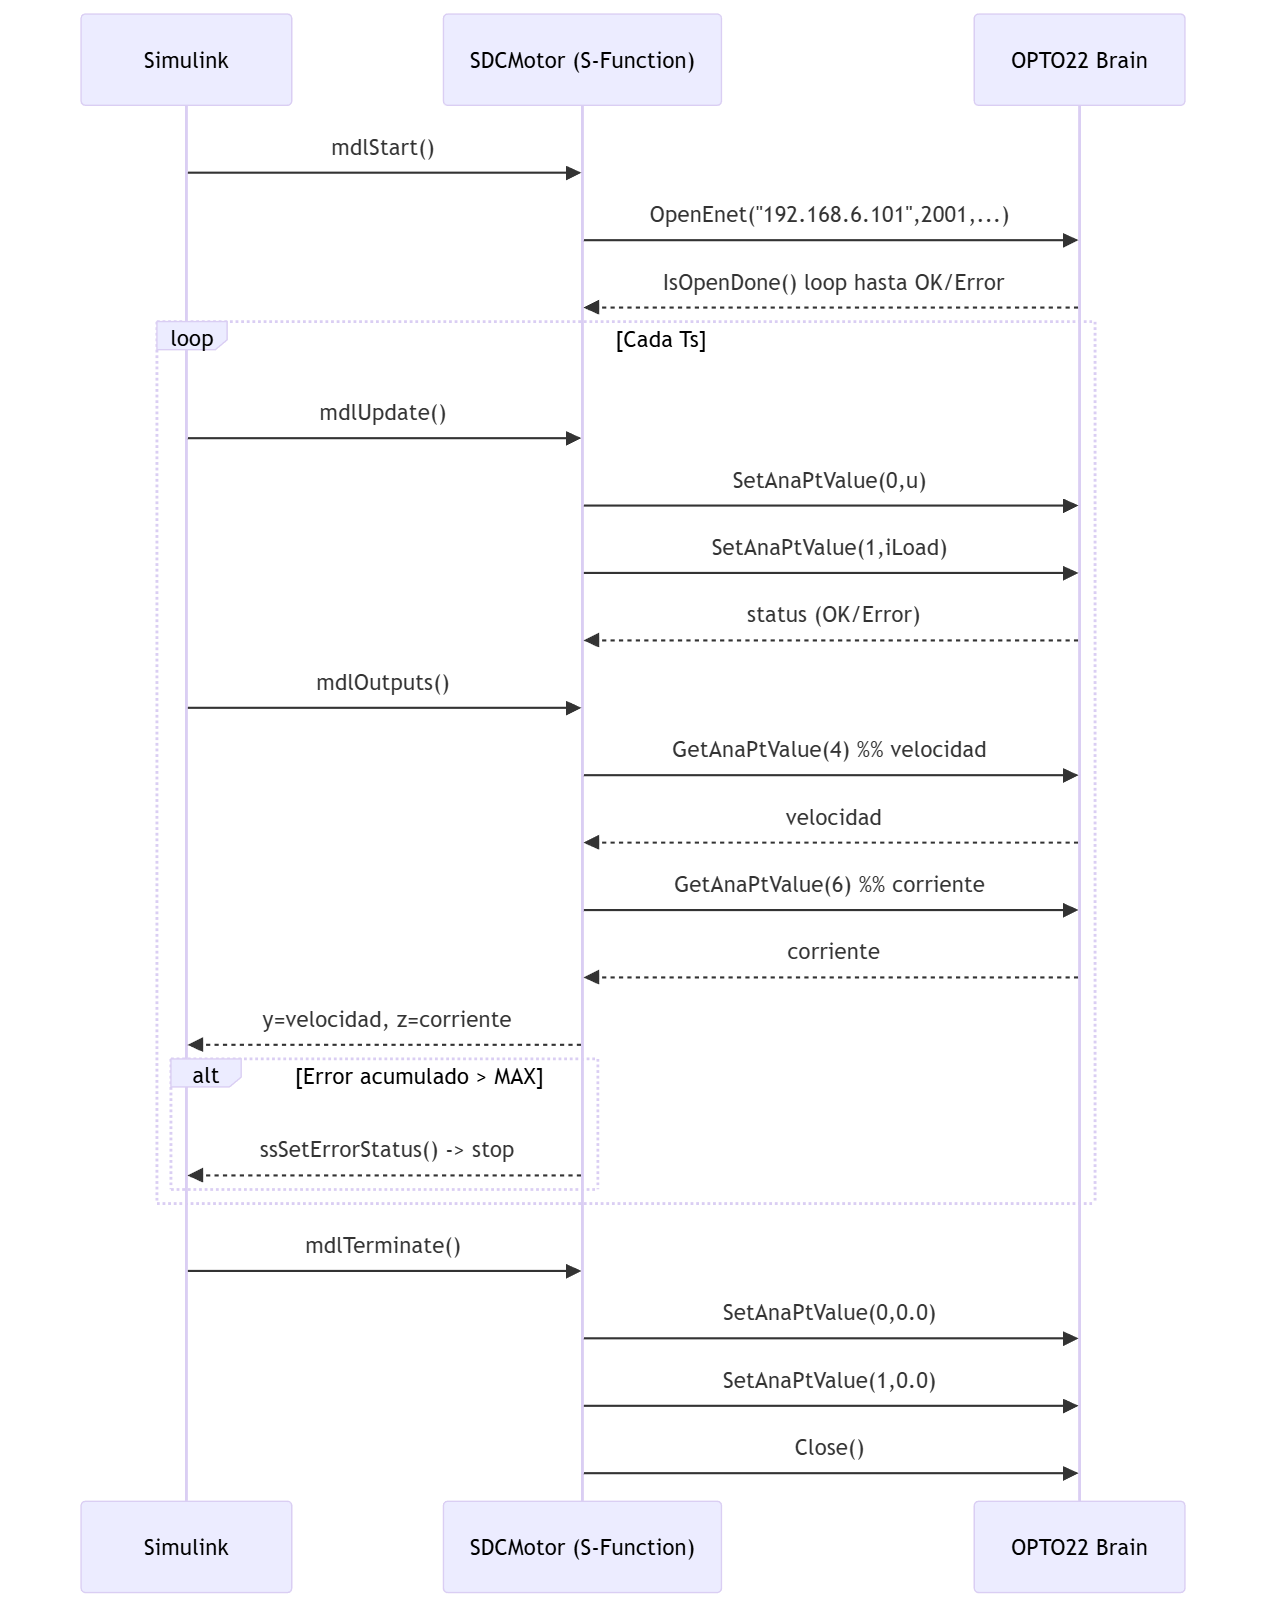
\includegraphics[width=0.7\textwidth]{img/SDCMotor/SDCMotor_diagram.png}
    \caption{Caption}
    \label{fig:SDCMotor diagram}
\end{figure}

\subsection{Consideraciones de integración y configuración}
\begin{itemize}
    \item \hl{\textbf{IP de computador HOST:} \textbf{PONER ESAS COSAS DE LA IP DEL PC ESPECIAL}}
    \item \textbf{IP fija en el código:} la dirección \texttt{192.168.6.101} está embebida. Para reutilización en distintas configuraciones de red, es recomendable parametrizar IP/puerto como parámetros del bloque.
    \item \textbf{Entradas Analógicas adicionales:} En la configuración actual del setup, solo se ocupan 2 de los 4 puntos de entrada del modulo  \texttt{SNAP-AIV-4} \cite{opto22_snap_aiv4}, pero habilitar puntos adicionales puede incrementar el overhead y prohibir el uso de tiempos de muestreo menores.
    \item \textbf{Mapa de canales:} los índices (0,1,4,6) asumen una asignación concreta de puntos analógicos en el OPTO22. Cualquier cambio de cableado/escala debe reflejarse en este mapa o, idealmente, parametrizarse.
    \item \textbf{Escalamiento físico:} este bloque transmite y recibe valores \texttt{float} sin aplicar conversión (p.ej., V$\leftrightarrow$RPM). Si se requiere trazabilidad metrológica, conviene documentar (y/o implementar) funciones de escala y saturación directamente en la simulación.
    \item \textbf{Robustez:} el umbral de errores (\texttt{MAX\_ERROR\_COUNT=5}) detiene la simulación. Esto es útil como medida de seguridad.
\end{itemize}

\newpage
\section{Consideraciones y Precauciones}
\label{sec:consideraciones_y_precauciones}

\subsection{Consideraciones y precauciones hardware}

Antes de energizar el banco de pruebas, se debe verificar que todas las conexiones de potencia y señal coincidan con los diagramas del montaje. En particular, es importante revisar la polaridad de las fuentes, la continuidad de las tierras de referencia y la correcta conexión de los terminales de armadura y campo de las máquinas de corriente continua.

La carga electrónica y las etapas de acondicionamiento deben operarse dentro de los rangos de tensión y corriente definidos durante el diseño. No se recomienda aumentar la corriente de carga sin supervisar la temperatura del transistor de potencia y del disipador, ya que una disipación excesiva puede dañar el componente o modificar el comportamiento del sistema durante los ensayos.

También se debe evitar manipular el cableado con el sistema energizado. Cualquier cambio en las conexiones del motor, generador, sensores o carga electrónica debe realizarse con las fuentes desconectadas y verificando posteriormente que no existan cortocircuitos entre alimentación, tierra y señales analógicas.

\subsection{Consideraciones para simulación en tiempo real con Simulink}
\label{subsec:simulink_consideraciones}

La ejecución del modelo en Simulink depende del rendimiento del computador y de la estabilidad de la comunicación Ethernet con el OPTO22. Por este motivo, se recomienda utilizar un tiempo de muestreo $T_s$ coherente con la capacidad real del sistema, evitando valores demasiado pequeños que puedan generar retrasos, pérdida de sincronismo o saturación del procesamiento.

Durante las pruebas, se debe limitar el uso de bloques de visualización como \emph{Scopes}, registros excesivos de datos u otros elementos que aumenten innecesariamente la carga computacional. Asimismo, se recomienda cerrar aplicaciones en segundo plano y mantener el computador dedicado exclusivamente a la ejecución del modelo mientras se realizan ensayos en tiempo real.

\subsection{Consideraciones y precauciones módulos OPTO22}
\label{subsec:opto22_consideraciones}

\subsubsection{Módulos de E/S utilizados}
El banco de pruebas se implementa con módulos SNAP de OPTO22:
\begin{itemize}
    \item \textbf{Dual Analog Output \texttt{SNAP-AOV-27}}: 2 canales de \emph{salida analógica de voltaje} bipolar, con rango nominal de \(-10\) a \(+10\)~VDC. Cada canal puede suministrar solamente \(\pm 5\)~mA de corriente de carga, por lo que \emph{no debe utilizarse como driver de potencia}. Ambos canales comparten referencia y \textbf{no están aislados entre sí}, aunque el módulo sí posee aislamiento respecto a otros módulos o dispositivos del rack. \cite{opto22_snap_aov27}
    \item \textbf{Quad Analog Input \texttt{SNAP-AIV-4}}: 4 canales de \emph{entrada analógica de voltaje}, configurables por canal en \(\pm 10\)~VDC o \(\pm 5\)~VDC. Los canales \textbf{no están aislados entre sí}. \cite{opto22_snap_aiv4}
\end{itemize}

\subsubsection{Límites eléctricos y protección del hardware OPTO-22}
Para evitar daños en los módulos y/o en la electrónica asociada, se deben respetar las siguientes restricciones:
\begin{itemize}
    \item \textbf{No exceder el rango de salida del \texttt{SNAP-AOV-27}}: asegurar que la señal de comando enviada desde Simulink se mantenga dentro de \([-10, +10]\)~V, idealmente con saturación explícita en el modelo.
    \item \textbf{No exigir corriente de carga mayor a \(\pm 5\)~mA por canal} en el \texttt{SNAP-AOV-27}. Si se requiere accionar una etapa de potencia, debe usarse un amplificador/buffer externo de alta impedancia de entrada (p.\,ej. etapa de acondicionamiento) para que el módulo no entregue corriente directa a la carga. 
    \item \textbf{Entradas del \texttt{SNAP-AIV-4}}: garantizar que las señales medidas no superen el rango configurado (\(\pm 10\)~V por canal).
    \item \textbf{Referencias/tierras}: dado que los canales no están aislados entre sí (entrada y salida), es crítico compartir referencias de señal de forma consistente y evitar lazos de tierra.
\end{itemize}

\subsubsection{Conexión de red}
Con el fin de minimizar la incertidumbre temporal (\emph{jitter}) y la latencia en el canal de comunicación, se recomienda establecer una conexión \textbf{directa} (Ethernet--RJ45) entre el \emph{Brain} OPTO22 y el computador que ejecuta la simulación. En lo posible, se debe evitar el uso de routers o switches intermedios, ya que introducen colas, procesamiento adicional y potenciales retransmisiones, aumentando la variabilidad del retardo entre paquetes.

Adicionalmente, se sugiere que el computador utilizado para la simulación opere en una red dedicada y, de ser viable, \textbf{sin acceso a Internet} durante la ejecución. Esto reduce tráfico de fondo (actualizaciones, sincronizaciones, servicios en segundo plano) y contribuye a mantener un canal de comunicación más estable, consistente y reproducible para el lazo de control en tiempo real.


\newpage
\section{Sensor de corriente}
\label{sec:sensor_de_corriente}


Antes de todo, se menciona que los diseños de PCB fueron hechos mediante el software EasyEDA y la impresión de las PCBs en las dependencias del lab. de electrónica. Por otra parte, para realizar la medición de corriente de armadura del motor, se elaboró una PCB como la que se muestra en la imagen xx,



La siguiente imágen \ref{fig:sCorriente} presenta la el diagrama esquemático completo del circuito. En cuanto al funcionamiento se describe asi: la corriente de armadura del motor se mide a través de un sensor LA 55-P, este sensor se aprecia en la figura \ref{fig:sensor}.

\begin{figure}[H]
    \centering
    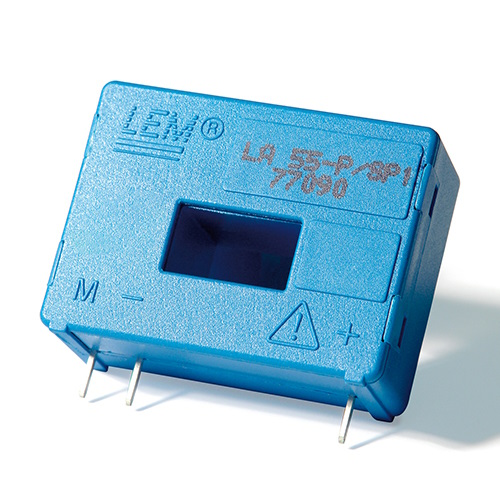
\includegraphics[width=0.4\linewidth]{img//SensorCorriente/sensor.jpg}
    \caption{Sensor LA 55-P}
    \label{fig:sensor}
\end{figure}

Para realizar su función, se atraviesa el cable cuya corriente va a ser medida por la abertura cuadrada que posee el sensor, de esta manera, el dispositivo entrega una corriente que se transforma a voltaje con una resistencia (R3 en el esquemático) y se amplifica mediante un circuito de amplificadores operacionales entregando un voltaje a la salida de la PCB (designado como 'SalidaSensorCorriente'), y posteriormente, este voltaje se digitaliza en el módulo OPTO-22 para ser comunicado al computador que realiza el control.

\begin{figure}[H]
    \centering
    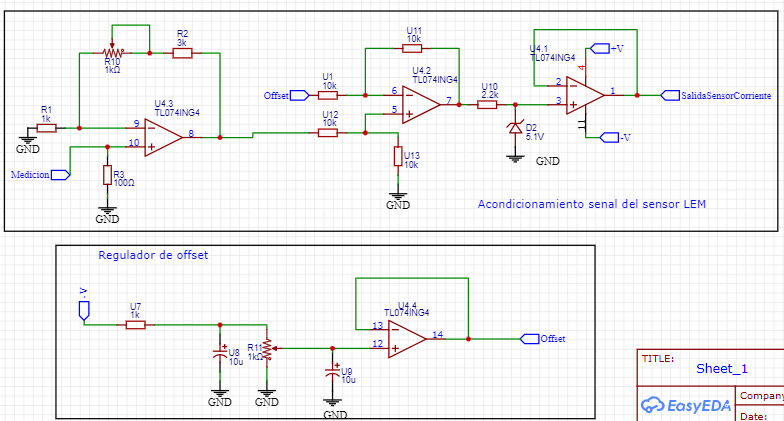
\includegraphics[width=0.75\linewidth]{img//SensorCorriente/sensorCorriente1.jpg}
    \caption{Acondicionamiento de la señal de corriente}
    \label{fig:sCorriente}
\end{figure}

Por ultimo, para realizar todas las funciones requeridas para acondicionar la señal de corriente, el circuito requiere de una fuente de alimentación simétrica como se ve en la fig. \ref{fig:fSimetrica}, el valor del voltaje de salida de la fuente es de +-12 Vdc.

\begin{figure}[H]
    \centering
    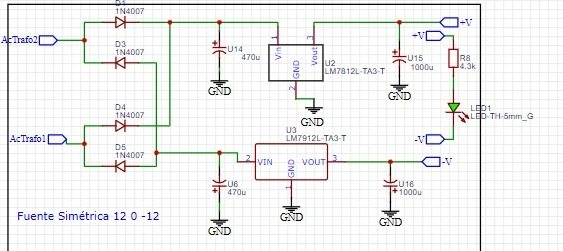
\includegraphics[width=0.75\linewidth]{img//SensorCorriente/fuenteSim.jpg}
    \caption{Fuente simétrica}
    \label{fig:fSimetrica}
\end{figure}

Cabe destacar que este módulo se alimenta gracias a un transformador simétrico de 12 Voltios RMS con un tap central, es decir, posee 3 cables de salida. Esto permite alimentar todas las PCB implementadas directamente desde la toma de 220 Voltios AC.



\newpage
\section{Carga electronica}
\label{sec:carga_electronica}


En esta sección se explica el diseño y funcionamiento del circuito diseñado para actuar como una carga electrónica controlada por voltaje. El propósito de este circuito, es ofrecer una condición de carga para la armadura del generador de manera que este ejerza un torque al motor DC, y que, además, esta carga pueda ser controlada desde el computador que está realizando el control del sistema. Se muestra a continuación el circuito ensamblado.



Para entender el funcionamiento del circuito, se debe saber que la parte más importante del mismo es el transistor BJT modelo TIP41C, ya que, este componente será el que disipe la mayor parte de la potencia eléctrica generada por el generador, por lo tanto, debe estar montado con un disipador térmico de buen tamaño. Además, se muestra el esquemático de la carga electrónica en la siguiente figura \ref{fig:cargaElec}.

\begin{figure}[H]
    \centering
    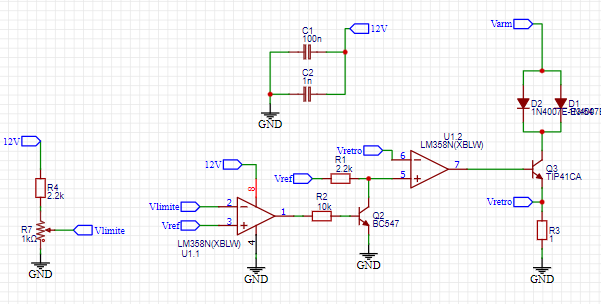
\includegraphics[width=0.75\linewidth]{img//cargaElectronica/cargaElec.jpg}
    \caption{Esquemático carga electrónica}
    \label{fig:cargaElec}
\end{figure}

Para realizar la función, el circuito se alimenta con 12 Volts, y el transistor se alimenta directamente de la armadura del motor, para el control de la corriente, el módulo recibe un voltaje de entrada, este voltaje de entrada es aplicado al Opamp (amplificador operacional), y este a su vez, lo aplica sobre la resistencia R3 del esquemático de la figura \ref{fig:cargaElec}, de esta manera, se produce una corriente igual a $\frac{Vcontrol}{R3}$, en muchas ocasiones se puede dejar R3 = 1 para que la corriente sea igual a Vcontrol, ademas, el transistor TIP41C es el encargado de proveer toda la corriente que pasar por la resistencia, por ende, el opamp termina siendo un controlador que no disipa mucha potencia (es importante que sea el modelo LM358). Por ultimo, la carga cuenta con 2 protecciones, 1) Un par de diodos D2 y D1 en la parte superior que impiden que se queme el transistor si es que se conecta en polaridad inversa la carga, y 2) el opamp 1.1 que impide que el voltaje Vcontrol aplicado a la resistencia R3 sea muy grande evitando que la carga pida mucha corriente, el valor de limite de corriente se puede ajustar a mano con el potenciómetro R7. Para garantizar un buen desempeño, se realizó una serie de pruebas a distintos voltajes y corrientes un con sensor de temperatura en el disipador para monitorear la temperatura del transistor TIP41C. Ver la tabla \ref{tab:datos}. Datos de la prueba: Tiempo de funcionamiento: 1 minuto, Temperatura ambiente: 28 grados celsius.

\begin{table}[H]
    \centering
    \caption{Temperaturas medidas (grados Celsius)}
    \begin{tabular}{|c|c|c|c|c|}
        \hline
        V, I & 0.2 A & 0.4 A & 0.6 A &  0.8 A\\
        \hline
        5 V & 28 & 29 & 31 & 30 \\
        \hline
        9 V & 29 & 31 & 33 & 34 \\
        \hline
        12 V & 32 & 33 & 38 & 37 \\
        \hline
    \end{tabular}
    \label{tab:datos}
\end{table}




\newpage
\bibliography{library}

\end{document}